% This file should be compiled as such: PdfLatex -> Bibtex -> PdfLatex (x2)

\documentclass[parskip=full-]{scrreprt}

\usepackage[utf8]{inputenc}

\usepackage{amsmath}
\newcommand\Rey{\mathrm{Re}}

\usepackage{amsfonts}
\usepackage{amssymb}
\usepackage{outlines}
\usepackage{xcolor}
\usepackage{geometry}

\usepackage{marginnote}
\renewcommand*{\marginfont}{\color{red}\sffamily}

\usepackage{lineno}
\renewcommand\linenumberfont{\normalfont\small\sffamily}
\linenumbers

\usepackage{graphicx}
\graphicspath{{../pics/}}

\usepackage{natbib}

\author{Jordan Wingenroth, Candace Yee, Justin Nghiem, and Laurel Larsen}

\title{Effective collector efficiency of sparse and dense arrays of cylindrical collectors in transitional turbulence}

\begin{document}

\maketitle

\chapter{Introduction}

TODO

\chapter{Methods}

\section{Theoretical Background}

In this study, we focus on direct interception of suspended particles by submerged vegetation. Direct interception is the adhesion of particles traveling along streamlines to the surfaces of collectors (e.g., plants). This is just one of several fluid dynamics mechanisms that act on suspended particles. Others include gravitational settling, inertial impaction, and diffusional deposition. Gravitational settling is the process of particles denser than water being drawn towards and coming to rest on the channel bottom. Inertial impaction and diffusional deposition are other means by which suspended particles can adhere to collectors. Inertial impaction occurs when particles possess momentum relative to streamlines, and diffusional deposition arises due to some combination of turbulence and Brownian motion.

Capture efficiency ($\eta=\frac{b_c}{d_c}$) is defined as the ratio between the upstream width ($b_c$) of the streamlines that encounter a collector and the collector's own diameter (\(d_c\)), which may be represented by an effective length in the case of non-cylindrical collectors (Figure 1).

\begin{figure}[htbp]
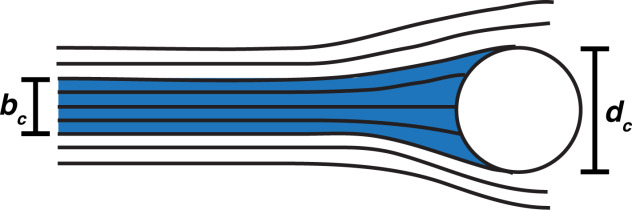
\includegraphics[width=10cm]{fauria particle capture efficiency diagram.jpg}
\centering
\caption[xxx]{Particle capture efficiency diagram (TODO: caption) \marginnote{Figure borrrowed from Fauria 2015. We should ask her permission before submitting, correct? Also, if we should make our own or swap in a different figure, let me know.}[-5cm]}
\end{figure}

Particle capture in transitionally turbulent flows (\(1<\Rey<1000\)), which occur commonly in the environments and on the length scales of aquatic macrovegetation, does not follow the analytical expressions involving Reynolds number, collector diameter, and particle diameter (\(d_p\)), derived for creeping flow. Hence, empirical estimates must be used. \citet{Palmer_2004} introduced a power law expression for estimating capture efficiency of cylindrical collectors, which takes the form \[\eta=C\Rey_c^{a}R^{b}\,,\] where \(\Rey_c=\frac{ud_c}{\nu}\), \(u\) is flow velocity, \(\nu\) is kinematic velocity, and \(R=\frac{d_c}{d_p}\) is the ratio between collector diameter and particle diameter (\(d_p\)). \(C\), \(a\), and \(b\) are empirically determined regression coefficients.

\section{Suspended Particle Concentration Model}

\[\frac{d\bar{\phi}}{dt} = -[\frac{Cv_s}{h}(1-E_r) + \eta^{\prime}ud_cI_c]\bar{\phi} = -k\bar{\phi}\]

\section{Experimental Methods}

\subsection{Materials}

Our experiment was conducted in a recirculating flume. Water was propelled by an electric pump through a rectangular pipe of gradually increasing hydraulic diameter (intended to avoid abrupt changes in velocity), through a honeycomb flow collimator, into a rectangular open channel containing our test section, then through another similar pipe feeding back to the pump (Figure XY). In the upper range of the pump's span, cavitation (i.e., taking on air bubbles) occured, which was accompanied by a distinct noise. By gradually increasing the pump's velocity while monitoring for sound, we determined that the pump stayed free of cavitation up to a rotation frequency well above 30 Hz, which was chosen as the maximum velocity for our experimental treatments. 

TODO: Flume floorplan figure 

We installed collectors in a removable array which was installed to fill a recessed well in the bottom of the rectangular channel. The perforated top of the array was covered with aluminum foil and gaps between the array and the upstream edge of the well was covered with an attached, flat, rectangular piece of aluminum in order to avoid irregularities in the channel's cross-sectional shape. Holes measuring approximately 2.5 cm in diameter were drilled in the array to hold the sediment traps.

\begin{figure}[htbp]
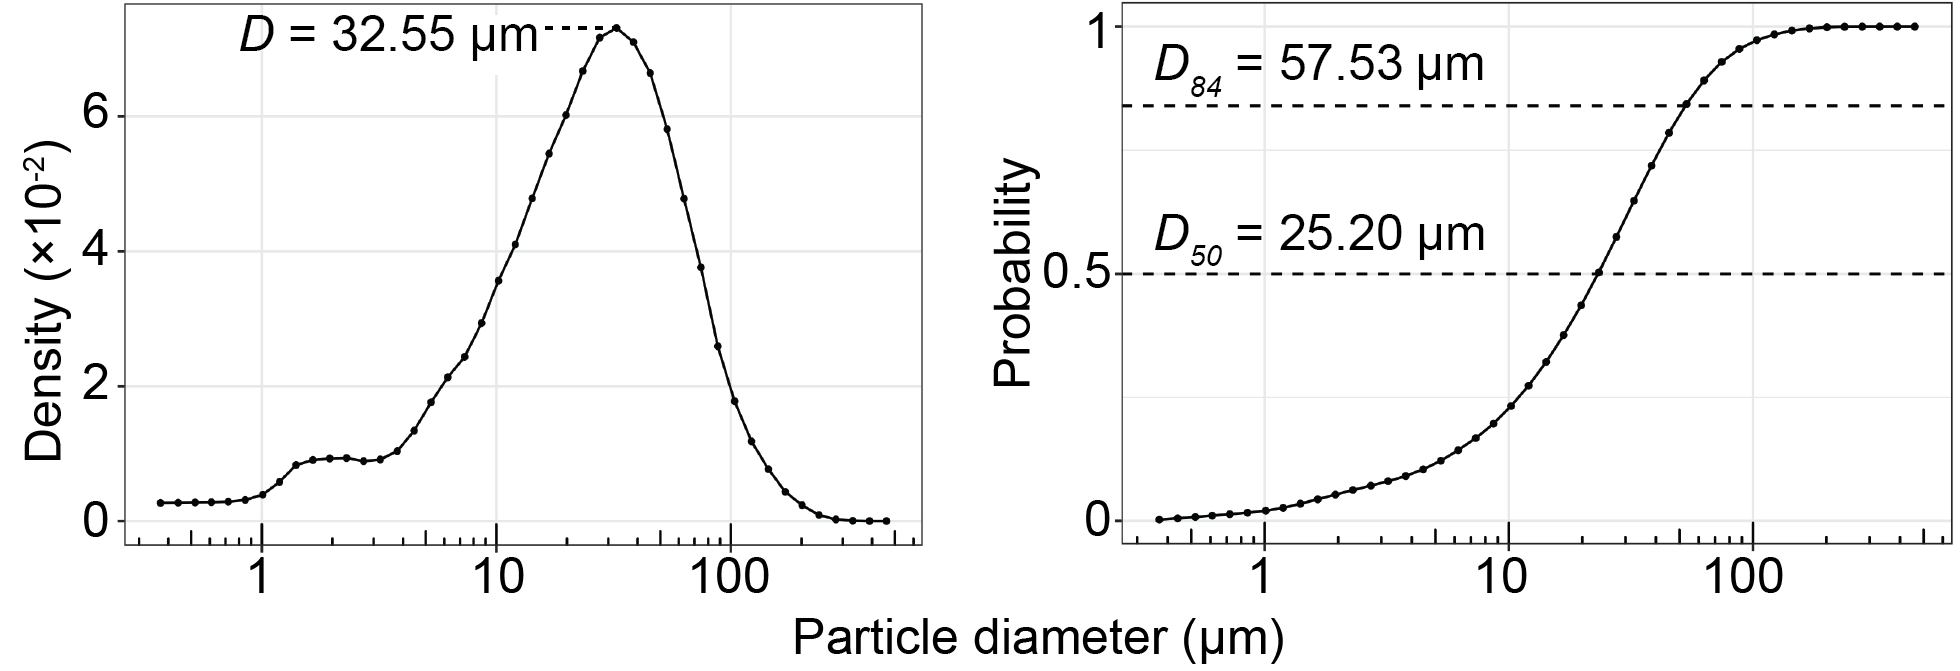
\includegraphics[width=10cm]{wf5-200sizedist.png}
\centering
\caption{Walnut shell particle size distribution (TODO: caption, crop out previous caption)}
\end{figure}

\subsection{Particle Concentration Run Protocols}

\subsection{Flow Characterization Run Protocols}

\section{Statistical Analysis}

\chapter{Results}

TODO

\chapter{Discussion}

TODO

The assumption that probability of retention (\(p_r\)) is 100\% when stems are coated with grease might be questionable based on our result that biofilm increased \(\eta\prime\) in comparison to greased dowels. The only other effect of biofilm that is readily apparent to me is perhaps increasing effective stem diameter (\(d_c\)). However, with our model for Reynolds number (\(\Rey_c \propto d_c\)), and both us and \citet{Fauria_2015} finding \(\eta\prime \sim -\Rey_c\), increasing stem diameter would be expected to have the opposite effect, unless I'm missing something.

\bibliographystyle{apalike}
\bibliography{refs}

\end{document}
